\chapter{Análisis de requisitos}

\textbf{Buscamos definir qué forma tendría una solución al
\hyperref[sec:problema_a_resolver]{problema a resolver}}.
Ideamos y negociamos junto al cliente el producto a entregar.
A partir de esta definición de producto obtenemos los requisitos
de la solución.

\section{Análisis del problema}

Acordamos con el cliente idear un producto teniendo como referencia la
\hyperref[sec:HU01]{HU01: Recuperación de histórico}%
\footnote{%
    Una historia de usuario describe una funcionalidad de un sistema de
    una forma casual y desde el punto de vista del cliente. A partir
    de las ideas que presenta se pueden ir extrayendo tareas para llegar
    al fin que describe.
}%
, ya que
no define una solución en concreta pero describe cómo interactuará
el cliente con el producto, qué espera obtener y cuál es su motivación.

\subsection{HU01: Recuperación de histórico} \label{sec:HU01}

{ \itshape Como operario quiero, dada una fecha pasada, poder consultar
en qué ubicación trabajé, durante cuánto tiempo, cuántos
árboles vibré y cuál fue el tiempo medio entre
vibraciones y vibrando, para poder demostrar ante un tercero
que he realizado un trabajo. }

\subsection{Plataforma hardware}

Nuestro cliente estima que esta característica únicamente debe implementarse
en su producto de gama más alta, los controles electrónicos con pantalla.
Los controles electrónicos con pantalla están compuestos por tres sistemas.

\begin{itemize}[noitemsep,nolistsep]
    \item \textbf{HMI}. Módulo que por medio de una interfaz gráfica muestra al usuario
          métricas acerca de la máquina. Se comunica con el control mediante un puerto
          serie asíncrono.
    \item \label{sec:joystick_con_control} \textbf{MF2424v1.2 (Joystick con control)}. Módulo de potencia que decide qué acción realizar
          según las lecturas de un joystick. Controla el sistema hidráulico del
          paraguas vibrador.
        \begin{itemize}[noitemsep,nolistsep]
            \item Microcontrolador Renesas RA6M1.
            \begin{itemize}[noitemsep,nolistsep]
                \item Arm® Cortex®-M4.
                \item 8kiB Data FLASH.
                \item 128kiB SRAM.
                \item USB2.0 FS.
            \end{itemize}
            \item Conexión mediante UART a un módulo HMI propietario.
            \item Conexión mediante SPI a FRAM Fujitsu \texttt{MB85RS16NPNF-G-JNERE1} de 4kiB.
            \item Posibilidad de conexión mediante SPI a un segundo módulo SOIC-8 que utilice la misma huella que la PCB.
            \item CAN 2.0.
        \end{itemize}
    \item \textbf{MFSV (GNSS con lectura de sensores)}. Módulo que difunde en un bus CAN la
          lectura de sensores 4-20mA, frecuencia de pulsos de entrada,
          geolocalización y fecha y hora UTC.
\end{itemize}

El único sistema que podría permitir almacenar grandes cantidades de datos es la MF2424.

\subsection{¿Qué datos almacenar?}

Almacenar los datos en bruto nos permitiría poder realizar análisis sobre estos en un futuro.
Sin embargo, dada la incertidumbre del cliente acerca de la utilidad que tendría tener estos
datos y dado que quiere abaratar costes de desarrollo ya que no es una característica
que haya sido muy demandada, consideramos suficiente almacenar por cada día de trabajo el
resultado de las estadísticas que se piden en la \hyperref[sec:HU01]{HU01}.

\subsection{¿Cómo recuperamos los datos?}

Nuestro cliente propone desarrollar una aplicación móvil donde recuperar y consultar los datos
del Joystick con control. Aunque tendríamos más capacidad de mostrar información acerca de los
datos opinamos que sería una solución muy compleja para un problema tan simple.
Después de considerar los costes asociados al desarrollo, publicación
y mantenimiento de la aplicación, el encarecimiento que tendría el Joystick con control
al tener que desarrollarle una solución de comunicación inalámbrica y todos los pasos que
debería seguir el operario para recuperar la información, el cliente marca la solución como inviable.

Nosotros proponemos extraer los datos por medio de una memoria USB. Aunque potencialmente la solución
podría ser más económica y el proceso para el operario más simple esta solución tendría otros
desafíos, como es el poder asegurar la validez de los datos, el cambio del diseño de la caja y de
la MF2424 para soportar escribir datos sobre una memoria USB.

Por último, pensamos en mostrar la información por medio de nuestro HMI. Nuestro HMI tiene limitaciones
acerca de cuántos datos puede mostrar y de cómo se muestran los datos pero permitiría desarrollar una
interfaz gráfica suficiente para el propósito. Esta solución es la más económica
y el procedimiento para recuperar los datos es muy simple. Nos decantamos por esta opción.

\begin{figure}[!b]
    \centering
    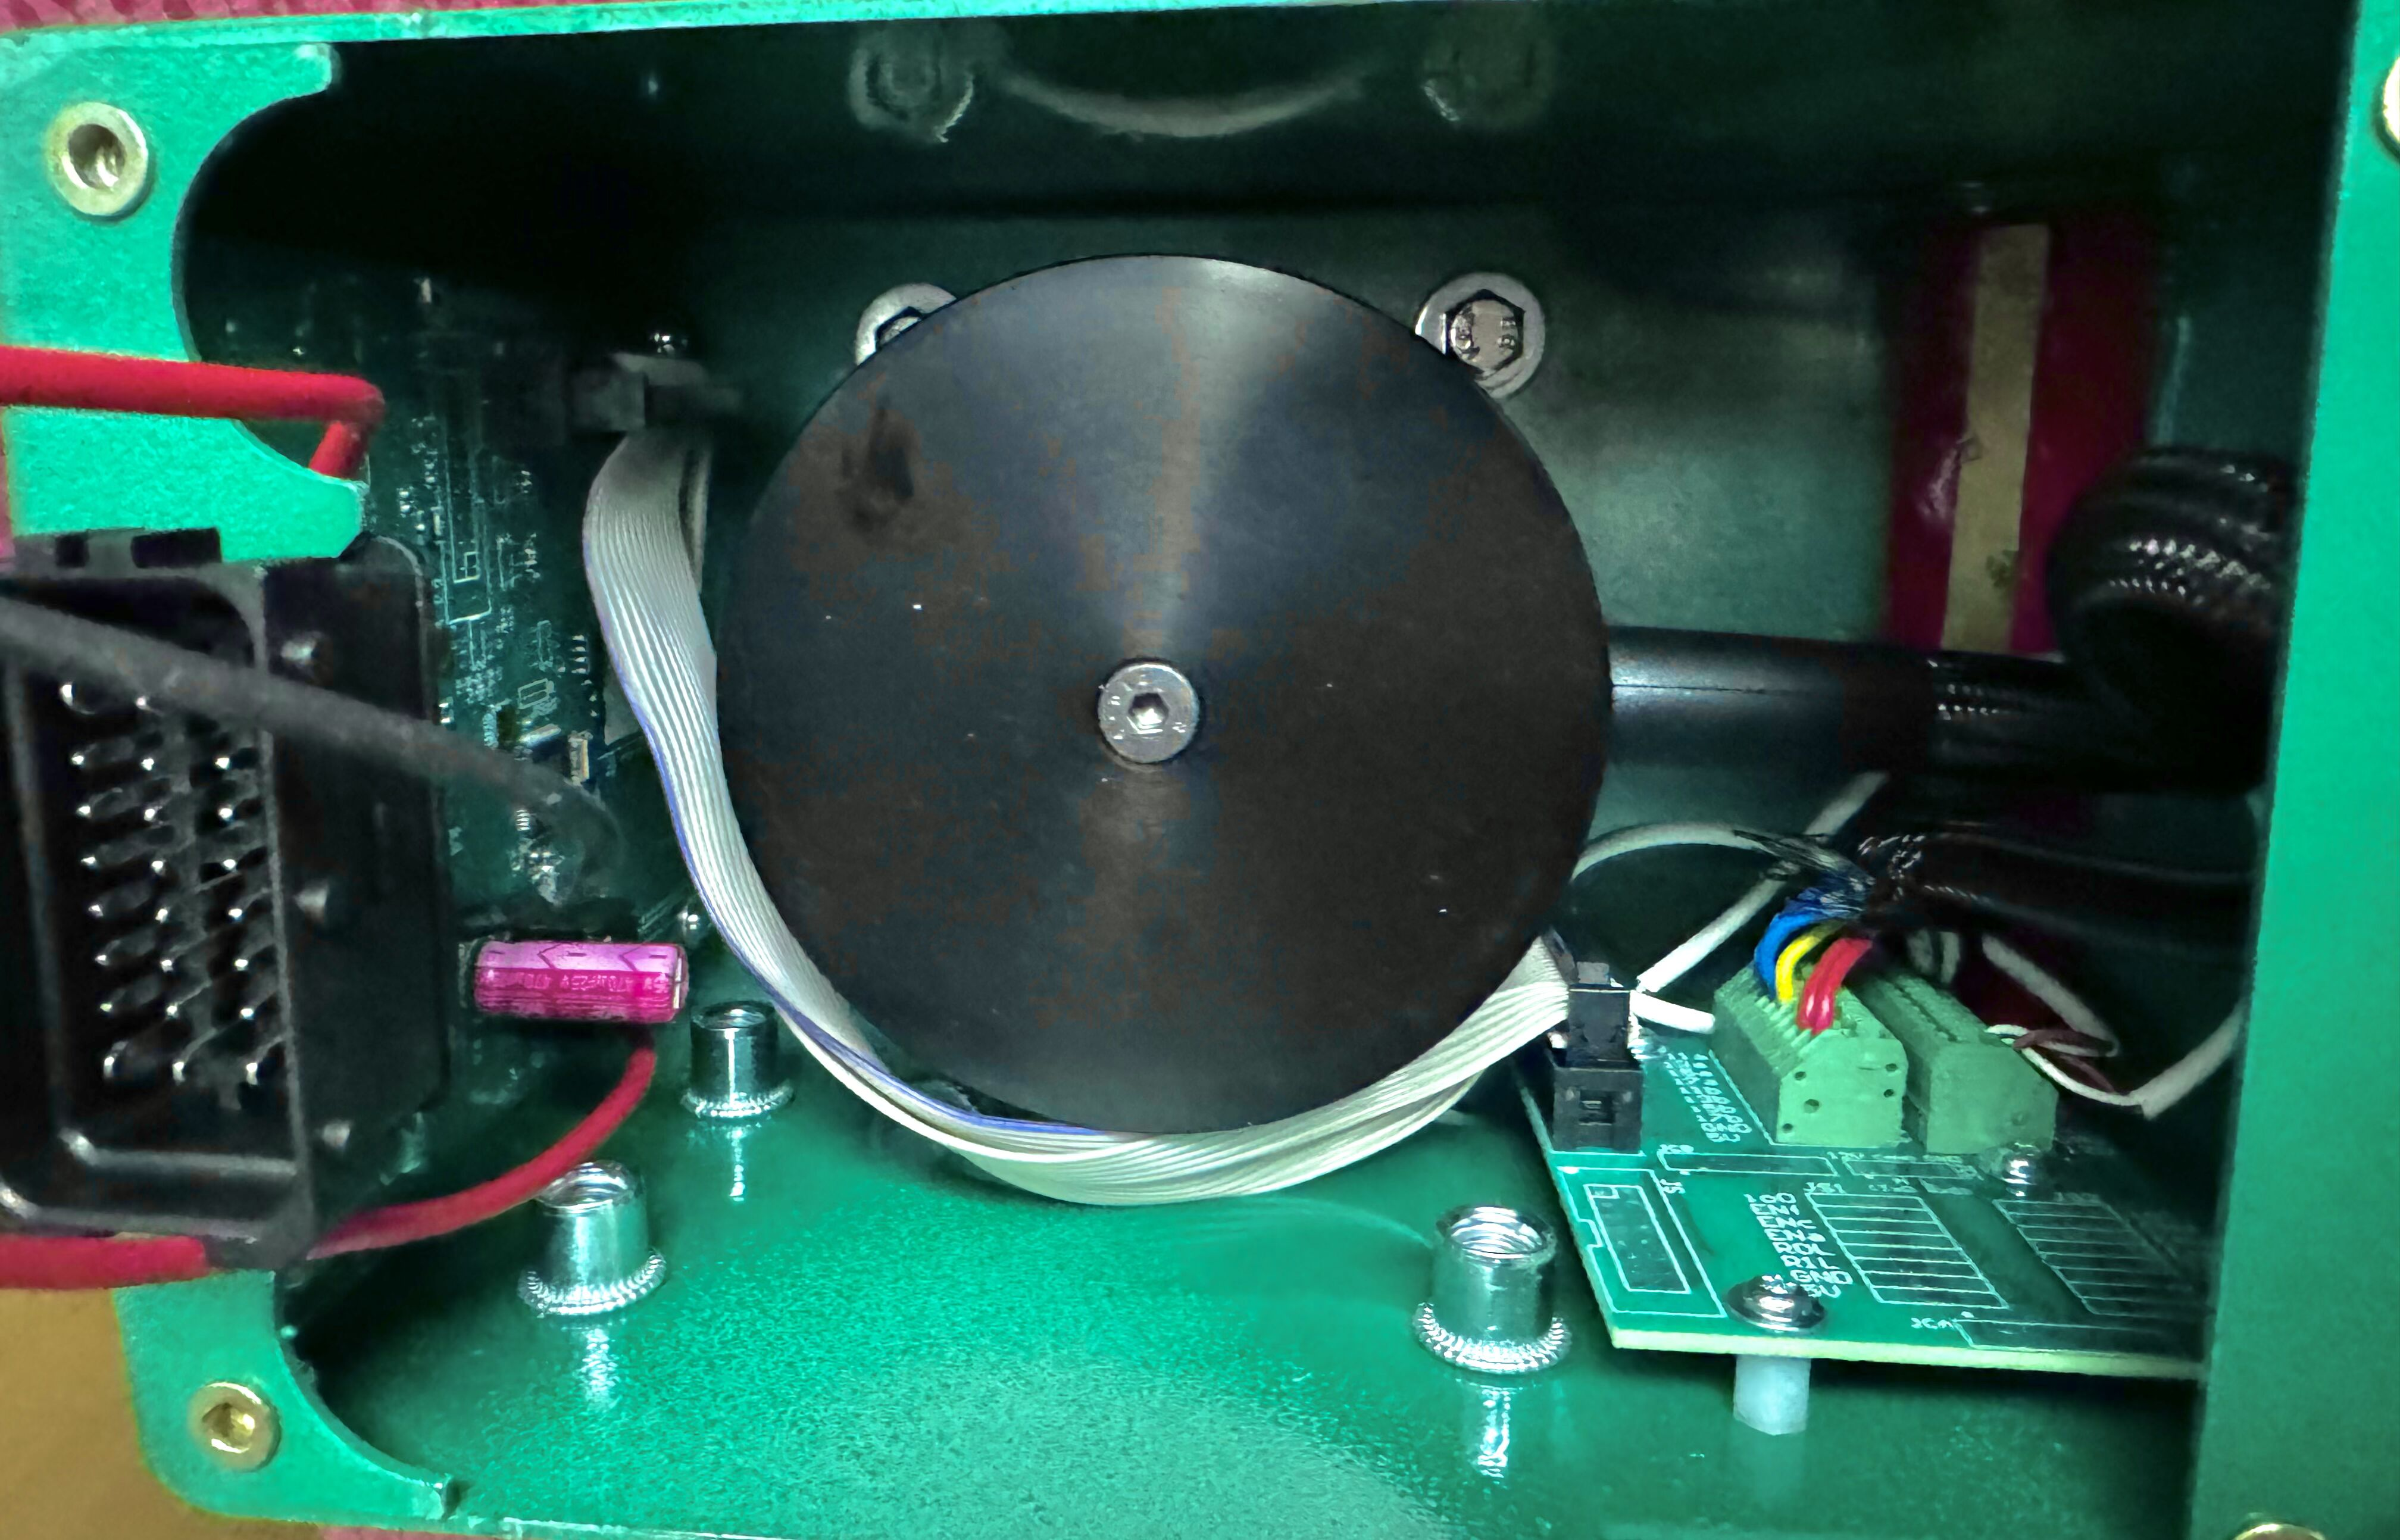
\includegraphics[width=\textwidth]{montaje_joystick_con_control.jpg}
    \caption{\textit{Sistema \hyperref[sec:joystick_con_control]{Joystick con control.}} \textit{Tenemos de
    izquierda a derecha la tarjeta MF2424, un Joystick digital y una tarjeta adaptadora.}
    \textit{La placa MultiFunción2424 alimenta las electroválvulas del
    sistema hidráulico según la secuencia de estados del Joystick por medio de reglas Software.}}
\end{figure}

\subsection{¿Cuánto almacenamiento necesitaremos para almacenar los datos?}

Desglosamos los datos que queremos almacenar de forma persistente y sumamos los bytes que sumarían.

\begin{itemize}[noitemsep,nolistsep]
    \item \textbf{El año, el mes y el día} puede almacenarse como el tipo \texttt{time\_t}, que en nuestra
        plataforma son los segundos desde el epoch.
        Mediante la función \texttt{gmtime\_r} y \texttt{mktime} podemos traducir de
        segundos a fecha y viceversa. Si utilizamos un tipo de 32 bits sin signo el sistema funcionaría
        correctamente hasta el año 2106 aproximadamente. Si utilizamos uno de 64 bits no tendríamos fecha
        de expiración.
    \item \textbf{La latitud o la longitud} pueden almacenarse como el tipo \texttt{float}%
    \footnote{Asumimos que el software se ejecutará en una plataforma que implementa el tipo como
    un número en coma flotante tal y como define el IEEE-754, como es nuestro caso con el RA6M1 \cite{renesas:RA6M1}.}%
    . Es suficiente al tener una precisión superior a los 10m.
    \item \textbf{El número de árboles vibrados} puede almacenarse como el tipo \texttt{uint16\_t}. Es
        suficiente al ser el número de valores significativamente mayor al que se puede trabajar en un
        día, que son 400 árboles aproximadamente.
    \item \textbf{El tiempo de vibración} puede almacenarse como el tipo \texttt{uint16\_t}. La vibración nunca
        es superior a 20 segundos y queremos hacer medias con precisión de la centésima del segundo. Por lo que
        podríamos almacenar medias de hasta 6553.5s, que no se darán.
    \item \textbf{El tiempo entre árboles} pueden almacenarse como el tipo \texttt{uint16\_t}. El tiempo
        entre árboles requiere una media con precisión de la centésima, y el tiempo máximo para que contabilice
        si seguimos trabajando es de 10 minutos, menos de los 109 minutos que tendríamos con el valor máximo
        de 6553.5s que podríamos almacenar.
\end{itemize}

El paso del tiempo es monótonamente creciente, por lo que podemos almacenar los
datos consecutivos en memoria desde la fecha del registro más antiguo al registro
más nuevo.

Gracias al almacenamiento ordenado y el hecho de que el acceso a la FRAM no ofrece
penalizaciones por localidad de la memoria%
\footnote{Aunque sí que cada consulta tiene una pequeña de sobrecarga en tanto
que tenemos que indicar la operación a realizar y una dirección de memoria.}
podríamos recuperar cualquier registro en tiempo $c \cdot log_{2} n$, con $c$
el tiempo que tardamos en recuperar la fecha del registro y $n$ el número de
registros almacenados en memoria.

En total ocuparíamos 32 bytes, de los cuales 10 irían destinados a \textit{padding}.
\hyperref[table:almacenamiento]{En esta tabla} describimos la disposición que tendrían un registro
de los datos en almacenamiento persistente.

\begin{table}[H]
    \centering
    \begin{tabular}{|l|l|l|}
        \hline
        Fecha                        & uint64\_t & Segundos desde el \textit{epoch} \\ \hline
        Latitud                      & float & Coordenadas decimales \\ \hline
        Longitud                     & float & Coordenadas decimales \\ \hline
        Número de árboles vibrados   & uint16\_t & Árboles \\ \hline
        Tiempo medio de vibración    & uint16\_t & Centésimas de segundo \\ \hline
        Tiempo medio entre árboles   & uint16\_t & Segundos \\ \hline
        \textit{Padding}             & uint16\_t &  \\ \hline
        \textit{Padding}             & uint32\_t &  \\ \hline
        \textit{Padding}             & uint32\_t &  \\ \hline
    \end{tabular}
    \caption{Estructura para el registro de estadísticas propuesto para un día de trabajo.
    Añadimos \textit{padding} hasta llegar a los 32 bytes. Esto permite que en un futuro
    podamos meter hasta 10 bytes más de información por registro sin afectar a la capacidad
    de almacenamiento, ya que tenemos capacidad de almacenar registros durante más de 44 años.}
    \label{table:almacenamiento}
\end{table}

\subsection{¿Cuánta memoria necesitaremos para almacenar un día de trabajo?}

Tanto la fecha como el número de árboles es inmediato. Son sus correspondientes tipos.

Para calcular las medias existen algoritmos estables numéricamente, de forma que como mucho
tendríamos que conocer el valor de la media anterior y el número de vibraciones o el número
de árboles, según corresponda.

\subsection{¿Qué dispositivos de almacenamiento utilizaríamos para el almacenamiento de los datos?}

Podemos utilizar cualquier tecnología que comparta la disposición de patillas con el módulo \linebreak \texttt{MB85RS16NPNF-G-JNERE1},
ya sea SOIC-8 o SOP-8. Consideramos módulos FRAM y FLASH.

Ambas tecnologías tienen sus propias ventajas. La tecnología FLASH permite mayor densidad de información,
aunque la escritura en los bloques tiene una vida limitada. La tecnología FRAM es más cara, pero permite
escribir y leer direcciones arbitrarias y el número de escrituras y lecturas es más que suficiente para la vida
útil de un producto.

Aunque un módulo FLASH compatible como puede ser el Infineon Technologies \linebreak \texttt{S25FL128LAGMFB013} tiene un
precio para 10 unidades de 2,59€/u. y un módulo FRAM de 512kiB tiene un precio para 10 unidades de
8,17€/u., en principio nuestro cliente no espera vender esta tecnología a más de 20 equipos este primer año.
Desconocemos la tecnología, y desarrollar un controlador (o adaptar el que nos ofrece Infineon) para esta tecnología
encarecería el desarrollo, tanto en tiempo como en coste, comparado con el controlador de las FRAM que ponemos como ejemplo.

Consideramos como suficiente la memoria FRAM Fujitsu Semiconductor \linebreak \texttt{MB85RS4MTYPF-G-BCERE1} de 512kiB,
que permite almacenar registros para más de los 5 años que nos pide el cliente.

\subsection{¿Cómo interactuaría el usuario con el sistema?}

Quien desarrolla la interfaz gráfica nos indica que la capacidad
expresiva de esta es mínima. Tenemos que adaptar la capacidad
expresiva del diseño a las capacidades del soporte software y
hardware del vendedor de las pantallas que se eligieron para el proyecto
del que es parte este módulo.

La comunicación entre módulos la hacemos mediante estructuras de datos.
Según el estado de estas estructuras de datos nuestro programa y el de
nuestro colaborador saben que hacer. Por experiencia sabemos que esta
es la forma más efectiva para ambos para desarrollar.

Negociando con el colaborador llegamos a la interfaz que describimos
en \hyperref[fig:interfaz_gráfica]{las figuras dedicadas a la interfaz
gráfica}.

\begin{figure}[!b]
    \begin{minipage}[b]{0.48\textwidth}
        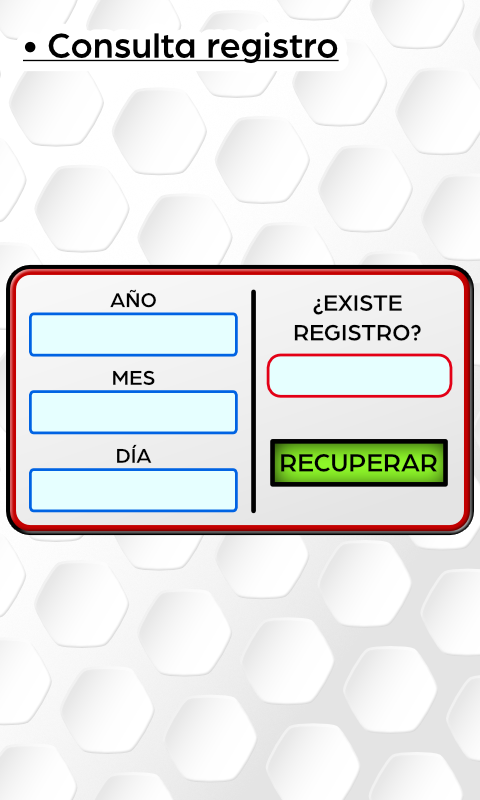
\includegraphics[width=\textwidth]{pantalla_consulta_registro.png}
        \caption{Interfaz para consultar un registro. El usuario puede
        introducir numéricamente por medio de un teclado emergente al pulsar
        sobre los cuadrados azules la fecha que quiere consultar. Una vez
        introducida se muestra el texto ``SÍ'' o ``NO'' en el campo ``¿EXISTE REGISTRO?''.
        En caso de que exista el registro, al pulsar sobre el botón ``RECUPERAR'',
        navegamos a la pantalla ``Registro''.}
    \end{minipage}
    \hfill
    \begin{minipage}[b]{0.48\textwidth}
        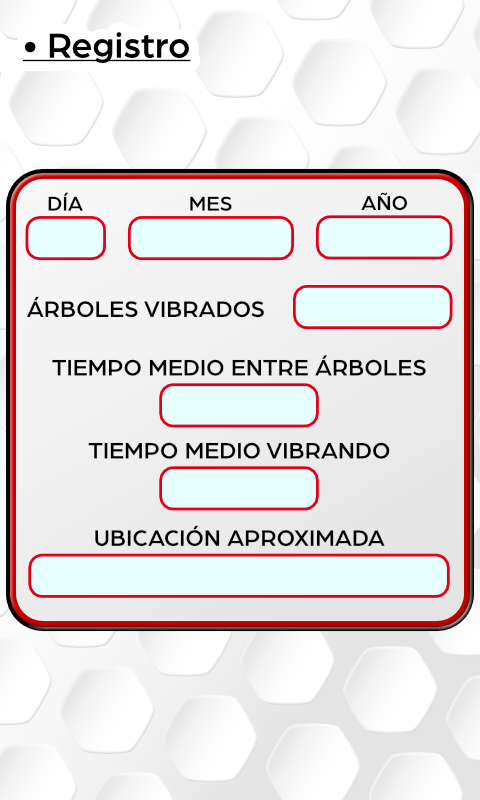
\includegraphics[width=\textwidth]{pantalla_registro.png}
        \caption{Interfaz para visualizar los datos de un registro. Accedemos
        a esta pantalla a partir de la pantalla ``Consulta registro''. El día
        se muestra como número, el mes como texto y el año como número.
        Los árboles vibrados como entero, los tiempos como segundos con 
        precisión de la centésima y con la unidad ``s'' y la ubicación
        aproximada en formato DMS (\textit{\textit{Degrees, Minutes, Seconds.}}).}
    \end{minipage}
    \label{fig:interfaz_gráfica}
\end{figure}

\section{Definición del comportamiento del sistema}

Describimos en forma de requisitos funcionales y no funcionales el
comportamiento que queremos que tenga el sistema. De esta forma, al resumir
la información que analizamos en la sección anterior, tenemos una
idea general acerca de este.

Los requisitos definitivos se codifican en forma de tests, por lo que
esta síntesis sólo es una ayuda inicial.

%\subsection{Cuestiones arquitectónicas}

\subsection{Reacción del sistema a partir de los eventos del control}

\subsubsection{RNF01: Límite de tiempo procesando eventos}

Cualquier llamada bloqueante al sistema no tarda más de 25ms
en terminar su proceso para asegurar el correcto funcionamiento del
resto de módulos que componen la solución del control.

\subsubsection{RF01: Detección del evento \textit{vibrar árbol}}

El sistema declara y define una función pública a invocar
de forma recurrente que tiene como parámetros los datos que definen
a un evento.

Un evento debe tener la información suficiente para deducir
las estadísticas solicitadas en el HMI (RF03).

El sistema identifica cada vez que hemos vibrado un árbol.

Hemos vibrado un árbol en el momento en que abrimos pinza en
la secuencia de movimientos \textit{cerrar pinza, vibrar y abrir pinza}.
Entre medias de esta secuencia, o durante, pueden ocurrir otros
movimientos.

Ante el evento de vibrar un árbol el sistema invoca a una función
del mismo para analizar y registrar los datos del evento. (RF02)

Es muy difícil que este requisito cambie puesto que se basa en el
funcionamiento del paraguas vibrador.

\subsubsection{RF02: Procesamiento del evento \textit{vibrar árbol}}

El sistema al detectar el evento \textit{vibrar árbol} recupera
el estado actual del registro del día en que nos encontramos.
A partir de este y junto a los datos del evento decide el nuevo
estado en que debe estar el registro, ordenándolo almacenar
sobrescribiendo el anterior.

Este requisito puede que cambiase en el caso de que los requisitos
de la estructura de datos subyacente cambiasen (RF04) (RF05) (RF06).

\subsection{Recuperación de información por parte del usuario}

\subsubsection{RF03: Consulta de un registro por un usuario}

Un usuario puede indicar en el HMI un año, un mes y un día.
Si no existe un registro para este día se indica.
Si existe muestra la fecha, la ubicación aproximada del trabajo,
el número de árboles vibrados, el tiempo medio entre vibraciones
y el tiempo medio entre árboles.

El usuario puede sufrir de dificultades a la hora de leer,
debido a vista cansada o similares. Además, la pantalla se
utilizará a plena luz del día.

Este requisito muy probablemente cambie si los usuarios no
lo perciben intuitivo.\footnote{
    Para evitar realizar esfuerzo innecesario, antes de implementar,
    lo ideal sería realizar un diseño y preguntar a personas que desconocen
    el propósito de la interfaz y cómo se interactúa con ella para
    qué sirve y cuál es su propósito, y comprobamos que interactuarían
    correctamente con ella, evaluando sus comentarios. Sin embargo,
    buscamos una solución suficiente para poder obtener feedback 
    del prototipo en el campo, ya que la campaña de recolección de la
    almendra ya ha empezado.
}

\subsection{Estructura de datos para almacenar los registros}

Estos requisitos sería fácil que cambiasen en el momento en que
utilizásemos otro tipo de soporte hardware para el almacenamiento
o acceso a la información.

\subsubsection{RF04: Recuperación de un registro}

El sistema recupera un registro dada una fecha de consulta.
El sistema conoce la posición en memoria del registro con la fecha
más antigua y el registro de la fecha más reciente (RF06).
En caso de no existir lo indica sin perturbar el flujo de ejecución.
Al recuperar el registro también devuelve información suficiente para
que (RF05) pudiera escribir datos sobre el registro.

La recuperación de un registro se realiza por medio de una búsqueda
binaria sobre las fechas que almacenamos en la FRAM.
Esta operación no modifica los datos contenidos en la FRAM.

\subsubsection{RF05: Escritura de un registro}

Dado un registro existente (RF04) (RF06) el sistema permite almacenar nuevos
datos en este registro.

\subsubsection{RF06: Creación de un registro}

Consideramos que una fecha es un año, un mes y un día.

Dada una fecha más reciente que cualquiera de las fechas almacenadas
el sistema crea un nuevo registro inicializada con esta nueva fecha
y con los datos a cero, actualizando la posición de memoria del registro
más antiguo y del más reciente.

En caso de no cumplir la precondición no crea un registro.

En caso de que no queden huecos para nuevos registros se sobrescribe
el más antiguo utilizando una política \textit{FIFO}.
